\documentclass[../../main.tex]{subfiles}

\graphicspath{{\subfix{../../immagini/}}}

\begin{document}

Le architetture di reti introdotte nei precedenti paragrafi risultano limitate in contesti in cui lavoro su insiemi di dati i cui esempi sono formati da elementi che non sono indipendenti tra loro: prendiamo come esempio un dataset in cui ogni esempio è un frase di lunghezza fissata, ovviamente con un dataset del genere potrebbero essere presenti frasi con lo stesso significato ma formulate in modo differente, e dunque con una sequenza di parole diversa; una rete feedforward, avendo parametri diversi per ognuna delle posizioni della frase, faticherebbe a riconoscere esempi con significati uguali, ma formulazioni differenti: ogni parola verrebbe essenzialmente considerata come indipendente rispetto alle parole precedenti e successive.

Quando ci si trova a lavorare con dataset di questo tipo spesso si preferisce utilizzare le \textit{reti ricorrenti} (RNN), \cite{rumelhart:errorpropnonote}. Caratteristica fondamentale di questa famiglia di reti è il fatto che gli strati del modello condividono gli stessi parametri, questo, oltre a portare ad un numero di parametri prefissato e non dipendente dalla lunghezze della sequenza, permette anche di dare importanza alla posizione, spesso chiamata timestamp, di un elemento. La condivisione dei parametri viene concretizzata in questo modo: ogni risultato in uscita alla rete è funzione dei risultati prodotti in uscita negli istanti precedenti, e ogni risultato viene calcolato utilizzando la stessa regola di aggiornamento applicata ai precedenti risultati.

L'esempio del dataset presentato poco sopra permette di mostrare un'altra caratteristica delle RNN: il fatto di condividere gli stessi parametri nei vari strati permette di avere lavorare su testi di lunghezza variabile, di fatto la rete mantiene in memoria una sola matrice di pesi che viene aggiornata ad ogni timestamp, di conseguenza può ricevere in ingresso testi con un numero di parole arbitrario (tutte le parole saranno però vettori aventi la stessa grandezza).\\
In linea teorica possiamo quindi avere reti ricorrenti che accettano in ingresso sequenze $(\boldsymbol{x}^{(1)}, \boldsymbol{x}^{(2)}, \dots)$ di lunghezza arbitraria, nella pratica però molte librerie che forniscono implementazioni di questa tipologia di reti permettono di avere solamente un numero fissato di strati, questa scelta viene giustificata dal fatto che in un dataset posso facilmente ricavare la lunghezza massima tra gli esempi, e nel caso di esempi di lunghezza inferiore posso semplicemente renderli più lunghi tramite il padding.

Per rappresentare una rete ricorrente è utile introdurre il concetto di \textit{grafo computazionale}: in un grafo di questo tipo ogni nodo indica una variabile, che può essere uno scalare, un vettore o una matrice, mentre un arco $(x,y)$ indica l'utilizzo della variabile $x$ in un'operazione che ha come risultato $y$.

Un grafo computazionale viene definito con una serie di operazioni base, operazioni più complesse vengono rappresentate come combinazioni di quelle base.

Formalmente posso rappresentare lo stato di un livello nascosto della rete ricorrente come:
\[\boldsymbol{n}^{(t)} = f(\boldsymbol{n}^{(t-1)}, \boldsymbol{x}^{(t)}, \boldsymbol{\Theta}),\]
dove $\boldsymbol{n}$ rappresenta lo stato del livello al tempo $t$ .\\
Posso rappresentare questa funzione ricorsiva tramite il grafo computazionale in Figura \ref{fig:computationgraph}.
\begin{figure}[H]
    \centering
    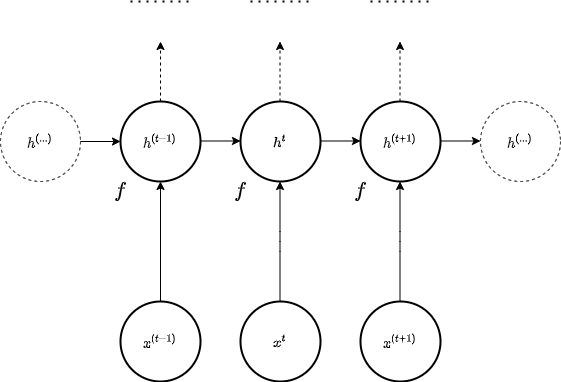
\includegraphics[scale = 0.4]{immagini/4_2/computation_graph.png}
    \caption{Esempio di grafo computazionale.}
    \label{fig:computationgraph}
\end{figure}

Definite le caratteristiche base di una rete ricorrente, possiamo combinare gli elementi a disposizione per andare a creare diverse architetture, alcune delle più frequenti sono riportate di seguito.

\begin{itemize}
    \item Reti ricorrenti che producono un risultato ad ogni istante di tempo ed hanno connessioni ricorrenti tra strati nascosti (Figura \ref{fig:RNNArch1}).
    \item Reti ricorrenti che producono un risultato ad ogni istante di tempo ed hanno connessioni tra il risultato al tempo $t-1$ e lo strato nascosto al tempo $t$ (Figura \ref{fig:RNNArch2}).
    \item Reti ricorrenti con connessioni tra strati nascosti e che producono un solo risultato al termine della sequenza (Figura \ref{fig:RNNArch3}).
\end{itemize}

\begin{figure}[H]
    \centering
    \begin{subfigure}[t]{0.49\textwidth}
        \centering
        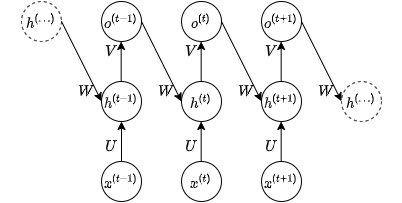
\includegraphics[width = \textwidth]{immagini/4_2/recnet2.png}
        \caption{}
        \label{fig:RNNArch1}
    \end{subfigure}
    \begin{subfigure}[t]{0.49\textwidth}
        \centering
        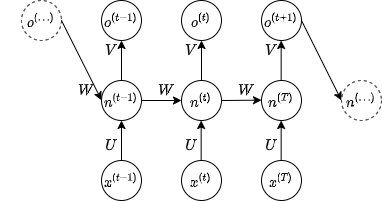
\includegraphics[width = \textwidth]{immagini/4_2/recnet.png}      
        \caption{}  
        \label{fig:RNNArch2}
    \end{subfigure}
    \begin{subfigure}[t]{0.49\textwidth}
        \centering
        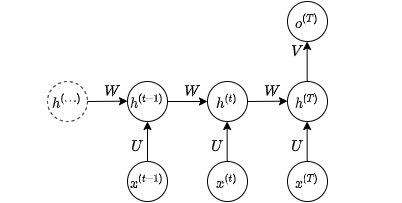
\includegraphics[width = \textwidth]{immagini/4_2/recnet3.png}  
        \caption{} 
        \label{fig:RNNArch3}  
    \end{subfigure}
    \caption{Esempi di possibili architetture di rete ricorrente. (a) Mostra una RNN con uscita ad ogni istante di tempo. (b) Mostra una RNN in cui l'uscita in ogni istante di tempo influenza lo strato nascosto dell'istante successivo. (c) Mostra una RNN con uscita solo all'ultimo istante di tempo.}
\end{figure}

Nel corso del tempo sono state proposte diverse implementazioni di questo tipo di architetture, quella da noi utilizzata negli esperimenti prende il nome di \textit{Gated Recurrent Unit} (GRU), la cui struttura viene introdotta nel paragrafo \ref{sec:strutturaRNN}.

\subsubsection{Apprendimento nelle reti ricorrenti}
Anche le RNN rientrano nella tipologia di modelli parametrici, l'apprendimento quindi avviene anche in questo caso cercando il miglior insieme di parametri sulla base degli elementi del training set; l'algoritmo più spesso utilizzato è ancora una volta la discesa del gradiente.

\begin{figure}[H]
    \centering
    \begin{subfigure}[b]{0.49\textwidth}
        \centering
        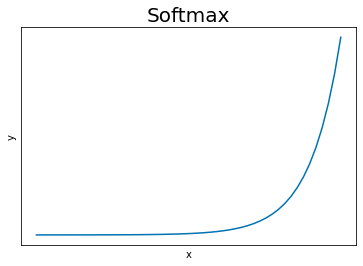
\includegraphics[width = \textwidth]{immagini/4_2/softmax.png}
        \caption{}
        \label{fig:softmax}
    \end{subfigure}
    \begin{subfigure}[b]{0.49\textwidth}
        \centering
        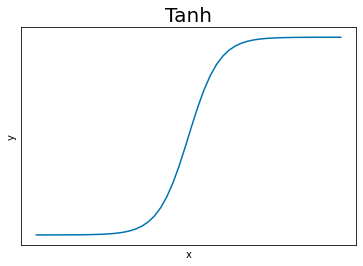
\includegraphics[width = \textwidth]{immagini/4_2/tanh.png}      
        \caption{}  
        \label{fig:tanh}
    \end{subfigure}
    \caption{(a) Grafico della funzione softmax. (b) Grafico della funzione tanh.}
\end{figure}

Per il calcolo del gradiente viene sfruttata una variante della  backpropagation, chiamata \textit{backpropagation through time} (BPTT), usata per far fronte ai problemi che sorgono dalla condivisione dei parametri. Prima di introdurre la BPTT è utile definire le equazioni che descrivono la forward propagation degli elementi in ingresso alla rete: il primo passo è l'inizializzazione dello strato nascosto $\boldsymbol{h}^{(0)}$ al tempo 0 , successivamente ad ogni istante di tempo il risultato delle rete viene calcolato come:
\begin{fleqn}[1cm]
    \begin{equation}
        \boldsymbol{a}^{(t)} = \boldsymbol{b} + \boldsymbol{W h}^{(t-1)} + \boldsymbol{U x}^{(t)},
    \end{equation}
    \begin{equation}
        \boldsymbol{h}^{(t)} = \mathrm{tanh}(\boldsymbol{a}^{(t)}),
    \end{equation}
    \begin{equation}
        \boldsymbol{o}^{(t)} = \boldsymbol{c} + \boldsymbol{V h}^{(t)},
    \end{equation}
    \begin{equation}
        \boldsymbol{\hat{y}}^{(t)} = \mathrm{softmax}(\boldsymbol{o}^{(t)}).
    \end{equation}
\end{fleqn}
Supponiamo quindi che la funzione di attivazione utilizzata sia una tangente iperbolica (tanh, figura \ref{fig:tanh}) e che il vettore dei risultati in un generico istante $\boldsymbol{\hat{y}}^{(t)}$ sia ottenuto applicando una funzione softmax (figura \ref{fig:softmax}) ai risultati della rete, di fatto ottenendo un vettore di probabilità; $\boldsymbol{a}^{(t)}$ e $\boldsymbol{o^{(t)}}$ rappresentano rispettivamente il vettore delle attivazioni dei neuroni dello strato nascosto e il vettore delle uscite, entrambi al tempo $t$. Infine, i parametri $\boldsymbol{U}$, $\boldsymbol{V}$ e $\boldsymbol{W}$ rappresentano le matrici di pesi rispettivamente tra livello d'ingresso e nascosto, livello nascosto e output e livello nascosto e livello nascosto all'istante successivo, $\boldsymbol{b}$ e $\boldsymbol{c}$ rappresentano invece i vettori di bias.

In questo caso utilizziamo la funzione di log-verosimiglianza come misura dell'errore commesso dal modello, in un generico istante $t$ quindi la perdita viene misurata come:
\[L^{(t)} = -\log(\boldsymbol{y}^{(t)}) = -\log(\mathrm{softmax}(\boldsymbol{o}^{(t)})),\]
mentre la perdita totale per una data sequenza di $\boldsymbol{x}$ con i relativi vettori $\boldsymbol{y}$ è data dalla somma delle perdite nei singoli istanti:
\[L(\{x^{(1)}, \dots, x^{(\mathcal{T})}\}, \{y^{(1)}, \dots, y^{(\mathcal{T})}\}) = \sum_t L^{(t)},\]
dove $\mathcal{T}$ indica l'ultimo timestamp.

Per il calcolo del gradiente (sfruttato poi per l'aggiornamento dei pesi) si ricorre anche in questo caso alla backpropagation. La caratteristica delle reti ricorrenti di avere pesi condivisi obbliga però a variare leggermente l'approccio base, adottato nei percettroni multistrato. Questa variante dell'algoritmo, come già accennato, prende il nome di backpropagation through time.
 
Il primo passo consiste nel calcolare i gradienti $\nabla_{\boldsymbol{N}}L$ dei nodi $\boldsymbol{N}$ interni del grafo computazionale:
\begin{fleqn}[0cm]
    \begin{align}
        \frac{\partial L}{\partial L ^ {(t)}} = \frac{\partial}{\partial L ^{(t)}} \sum_i L^{(t)} = 1,
    \end{align}
    \begin{align}
        (\nabla_{\boldsymbol{o}^{(t)}}L)_i = \frac{\partial L}{\partial o^{(t)}_i} = \frac{\partial L}{\partial L^{(t)}} \frac{\partial L^{(t)}}{\partial o^{(t)}_i} = 1 \cdot (\hat{y_i}^{(t)} - 1_{i,y^{(t)}}),
        \label{eqn:BPTT}
    \end{align}
    \begin{align}
        \nabla_{\boldsymbol{n}^{(t)}}L = \left(\frac{\partial \boldsymbol{h}^{(t+1)}}{\partial \boldsymbol{h}^{(t)}}\right)^\top (\nabla_{\boldsymbol{h}^{(t+1)}}L) + \left(\frac{\partial \boldsymbol{o}^{(t)}}{\partial \boldsymbol{h}^{t}}\right)^\top (\nabla_{\boldsymbol{o}^{(t)}}L),
    \end{align}
    \begin{align}
        \nabla_{\boldsymbol{h}^{(\mathcal{T})}}L = \boldsymbol{V}^\top \nabla_{\boldsymbol{o}^{(\mathcal{T})}} L .
    \end{align}
\end{fleqn}
Il risultato di \eqref{eqn:BPTT} viene giustificato ricordando come la funzione di perdita è definita e applicando la regola della catena:

\begin{flalign*}
    \frac{\partial}{\partial o_i^{(t)}} \log\left(\hat{y}^{(t)}\right) &= \left(\frac{\partial \log\left(\hat{y}_i^{(t)}\right)}{\partial \hat{y}_i^{(t)}} \cdot\frac{\partial \mathrm{softmax}\left(o_i^{(t)}\right)}{\partial o_i^{(t)}}\right),\\
    &= -\frac{1}{\hat{y_i}^{(t)}} \cdot \frac{e^{o_i^{(t)}} \left(\sum_j e^{o_j^{(t)}} - e^{o_i^{(t)}}\right)}{\left(\sum_j e^{o_j^{(t)}}\right)^2},\\
    & = -\frac{1}{\hat{y_i}^{(t)}} \cdot \left(\frac{e^{o_i^{(t)}}}{\sum_j e^{o_j^{(t)}}} \cdot \left(1 - \frac{e^{o_i^{(t)}}}{\sum_j e^{o_j^{(t)}}}\right)\right),\\
    & = -\frac{1}{\hat{y_i}^{(t)}} \cdot (\hat{y_i}^{(t)} (1 - \hat{y_i}^{(t)})) = (\hat{y_i}^{(t)} - 1).
\end{flalign*}
Sfruttando ancora una volta la regola della catena ed i risultati appena ottenuti possiamo ricavare i gradienti dei parametri del grafo:

\begin{fleqn}[0cm]
    \begin{align}
        \nabla_{\boldsymbol{V}}L = \sum_t \sum_i \left(\frac{\partial L}{\partial o_i^{(t)}}\right) \nabla_{\boldsymbol{V}}o_i^{(t)} = \sum_t (\nabla_{o^{(t)}}L) \boldsymbol{h}^{(t)^\top}
    \end{align}
    \begin{align}
        \nabla_{\boldsymbol{W}}L = \sum_t \sum_i \frac{\partial L}{\partial h_i^{(t)}} \nabla_{\boldsymbol{W^{(t)}}} h_i^{(t)} = \sum_t \text{diag} \left(1 - (\boldsymbol{h^{(t)}})^2\right) (\nabla_{\boldsymbol{h}^{(t)}}L)\boldsymbol{h}^{(t-1)^\top}
    \end{align}
    \begin{align}
        \nabla_{\boldsymbol{U}}L = \sum_t \sum_i \left(\frac{\partial L}{\partial h_i^{(t)}}\right) \nabla_{\boldsymbol{U}^{(t)}}h_i^{(t)} = \sum_t \text{diag} \left(1 - (\boldsymbol{h^{(t)}})^2\right) (\nabla_{\boldsymbol{h}^{(t)}}L )\boldsymbol{x}^{(t)^\top}
    \end{align}
    \begin{align}
        \nabla_{\boldsymbol{c}}L = \sum_t \left(\frac{\partial \boldsymbol{o}^{(t)}}{\partial \boldsymbol{c}}\right)^\top \nabla_{(\boldsymbol{o}^{(t)})}L = \sum_t \nabla_{\boldsymbol{o}^{(T)}} L
    \end{align}
    \begin{align}
        \nabla_{\boldsymbol{b}}L = \sum_t \left(\frac{\partial \boldsymbol{h}^{(t)}}{\partial \boldsymbol{b}^{(t)}}\right)^\top \nabla_{\boldsymbol{h}^{(t)}} L = \sum_t \text{diag}\left(1 - (\boldsymbol{h}^{(t)})^2\right)\nabla_{\boldsymbol{h}^{(t)}}L
    \end{align}
\end{fleqn}
Dove $\text{diag} \left(1 - (\boldsymbol{h^{(t)}})^2\right)$ indica la matrice diagonale contenente gli elementi $1 - (\boldsymbol{h^{(t)}})^2$ e corrisponde di fatto alla matrice delle derivate parziali della tangente iperbolica.\\
La notazione $\boldsymbol{W}^{(T)}$ indica il contributo della matrice di pesi al tempo $t$, in altre parole stiamo supponendo che i parametri tra uno strato nascosto e quello temporalmente successivo siano indipendenti tra loro, ciò permette di calcolare il contributo dei pesi in ogni istante di tempo per poi sommare tali contributi ottenendo il gradiente totale da utilizzare poi per l'aggiornamento.
\end{document}